\chapter{Attaques DDoS} 
\minitoc
\thispagestyle{empty}
\newpage
\section{Introduction}
Le Déni de service Distribué (DDoS) est l'attaque visant la disponibilité d'un service ou d'une ressource en la saturant de requête indésirable empêchant ainsi ses utilisateurs légitimes de l'utiliser. cette indisponibilité du service ou d'une ressource est mise en œuvre à travers les botnets.\\
Actuellement DDoS est probablement l'une des ménaces la plus courante et la plus dangereuse visant l'IoT vis à vis de l'explosion exponentielle du nombre d'objets connectes qui impliquent une augmentation colossale des Botnets à venir   \cite{refbotnet}.\\

À titre d'exemple : En 2007 l'Estonie \cite{refestonie} a été victime de la première plus grande attaque DDoS de l'histoire. l'attaque visait le système informatique du pays notamment ses sites gouvernementaux, ses banques et ses médias en les rendant indisponibles créant ainsi la panique et déclenchant une vaste d'émeute entre la population et les forces de l'ordre.\\

En octobre 2016 \cite{refddos} Dyn un important fournisseur de service de noms de domaine a été victime d'une vague d'attaque par déni de service distribuée. l'attaque était orchestrée à l'aide d'un logiciel malveillant appelé Mirai, les pirates se sont servis de ce programme pour créer un énorme botnet de 100000 objets connectés pour lanceur leur attaque. L'attaque a été extrêmement perturbatrice et a fait tomber les sites Web de plus de 80 de ses clients, notamment Amazon, Netflix, Airbnb, Spotify, Twitter, PayPal et Reddit. Les dommages causés par cette attaque auraient coûté 110 millions de dollars ainsi que la dégradation de la réputation du fournisseur. \\
	En 2018 github, une plateforme de développement à son tour était visée d'attaque DDoS, l'attaque a été maitrisée 10 min après \cite{refddos} grâce à la présence d'un système de protection d'attaque DDoS dans la plateforme.\\

	Une fois qu’un service est accessible via internet, il faut pouvoir estimer le risque de déni de service distribué. Un risque qui doit pas être laissé de côte. Car Il touche directement à la disponibilité des ressources qui peut être frustrant et coûteux aux entreprises. Un déni de service apparaît probablement lorsqu’il y a une surcharge des composants individuels du système d’information. Si cela est provoqué délibérément par une source externe, on parle alors d’attaque DoS, en l’occurrence, le remplissage d’un canal de communication ou une zone de stockage jusqu’à ce qu’on ne puisse plus l’utiliser.\\

Une méthode particulièrement efficace est lorsque le système est inondé de trafics illégitimes provenant de centaines, de milliers, voire de millions d’autres ordinateurs (souvent compromis). Ceci est connu sous le nom d’attaque DDoS.
	\section{Définition d’attaque DDoS}
	Une attaque par déni de service distribué (DDoS) est une tentative malveillante de perturber le trafic normal d'un serveur, d'un service ou d'un réseau ciblé en submergeant la cible ou son infrastructure environnante par un flot de trafic Internet. Les attaques DDoS atteignent leur efficacité en utilisant plusieurs systèmes informatiques compromis comme sources de trafic d'attaque. Les machines exploitées peuvent inclure des ordinateurs et d'autres ressources en réseau telles que les objets connectés. Par analogie, une attaque DDoS est comme un embouteillage obstruant l'autoroute, empêchant le trafic régulier d'arriver à sa destination souhaitée\cite{cloudflareddos}.\\

D’un point de vue technique, le terme déni de service est utilisé pour parler de l’incapacité du service à répondre aux trafics légitime durant l’attaque.
	\begin{figure}[H]
		\begin{center}
			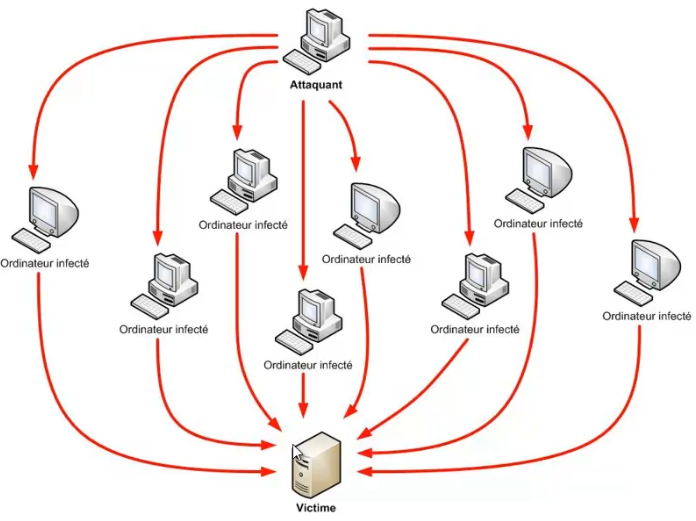
\includegraphics[height=10cm]{IMAGES/ORIGINALS/Architecture_attaque_DDoS}
		\end{center}
		\caption{Architecture d'attaque DDoS}
	\end{figure}
	\section{Principe de fonctionnement des attaques DDoS}
	Une attaque DDoS implique pour un attaquant de prendre le contrôle d'un réseau de machines en ligne afin de mener une attaque. Les ordinateurs et autres machines (comme les objets connectés) sont infectés par un malware, qui les transforme en bots (ou zombies). Le pirate contrôle alors à distance le groupe de bots, appelé un botnet.\\
	
	Un Botnet est une contraction des termes « robot » et « network » où chaque appareil infecté est appelé bot. Il fait référence à un groupe d'ordinateurs qui ont été infectés par des logiciels malveillants et qui sont tombés sous le contrôle d'un attaquant. Les botnets peuvent être conçus pour accomplir des tâches illégales ou malveillantes, notamment l'envoi de spam, le vol de données, les ransomwares, les clics frauduleux sur les publicités ou les attaques par déni de service distribué (DDoS).\\
	
	Une fois qu'un botnet a été mis en place, l'attaquant est en mesure de diriger les machines en envoyant des instructions de mises à jour à chaque bot via une méthode de contrôle à distance. Quand l’adresse IP d'une victime est ciblée par le botnet, chaque bot répond en envoyant des requêtes à la cible, ce qui peut saturer le serveur ou le réseau ciblé, entraînant un DoS pour le trafic normal. Étant donné que chaque bot est un périphérique Internet légitime, il peut être difficile de séparer le trafic d'attaque du trafic normal \cite{cloudflareddos}.
	\section{Catégories d’attaque DDoS}	
	Le nombre d’attaques par déni de service distribué s’est considérablement élevé au cours des dernières années. Ces attaques sont aujourd’hui fréquentes, et peuvent viser toute entité disposant d’un système d’information ou d’une infrastructure réseau connectée à Internet.\\
	
	Les botnets ciblent des vulnérabilités dans différentes couches d’interconnexion des systèmes ouverts et un vecteur d’attaque peut généralement être classé dans l’une des trois grandes catégories suivantes \cite{netscoutddos} : attaques par déni de service volumétriques, attaques par déni de service d’épuisement d’états TCP (TCP state-exhaustion attacks), et attaque de la couche d’application.
	\subsection{Attaques de la couche d’application}
	Généralement appelées attaques DDoS de couche 7 (en référence à la $7^{ième}$ couche du modèle OSI), le but est d'épuiser les ressources de la cible. Les attaques ciblent la couche où les pages Web sont générées sur le serveur et livrées en réponse aux requêtes HTTP. Une seule requête HTTP est peu coûteuse à exécuter côté client et peut coûter cher au serveur cible de répondre car le serveur doit souvent charger plusieurs fichiers et exécuter des requêtes de base de données afin de créer une page Web. Ces attaques sont souvent difficiles à empêcher car le trafic peut être difficile à détecter comme malveillant.\\
	La prolifération des dispositifs IoT non sécurisés au cours des dernières années a été avantageux pour les attaquants DDoS car il existe désormais un nombre presque illimité de dispositifs intelligents qui peuvent être utilisés comme botnet pour lancer des attaques de couche application plus avancées.

	\subsubsection{HTTP Flood}
	\begin{figure}[h]
		\begin{center}
			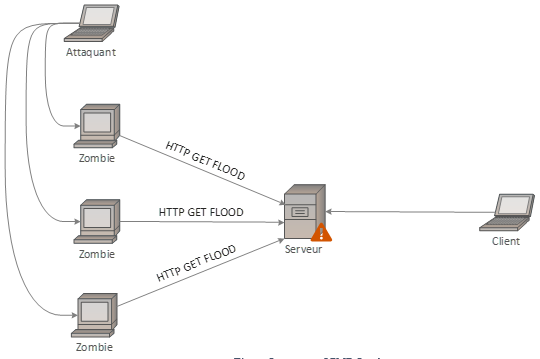
\includegraphics[height=7cm]{IMAGES/ORIGINALS/Attaque_HTTP_Flood}
		\end{center}
		\caption{Attaque HTTP Flood}
	\end{figure}

	Dans une attaque DDoS HTTP Flood, l'attaquant exploite des requêtes HTTP POST ou GET généralement légitimes pour attaquer une application ou un serveur Web. Les HTTP Flood n'utilisent pas de paquets malformés, de techniques de réflexion, ou d'usurpation et nécessitent moins de bande passante que les autres attaques pour faire tomber le serveur ou le site ciblé. L'attaque est plus efficace lorsqu'elle oblige le serveur ou l'application à allouer le maximum de ressources possible en réponse à chaque requête.
	\subsubsection{Slowloris}
	C’est un outil d’attaque écrit en Perl, créé par RSnake (Robert Hansen), une attaque de type DoS hautement ciblée, permettant à une machine de faire tomber un serveur en épuisant les ressources de connexion notamment des serveurs web sans affecter les autres services ou ports du réseau cible. Il y parvient en maintenant ouverts autant de connexions au serveur Web cible que possible. Il accomplit cela en créant des connexions au serveur cible, mais en n'envoyant qu'une demande partielle. Slowloris envoie constamment plus d'en-têtes HTTP, mais ne termine jamais une demande. Le serveur ciblé garde ouverte chacune de ces fausses connexions. Cela déborde finalement le pool de connexions simultanées maximum et conduit au refus de connexions supplémentaires de clients légitimes.\\
	
	Lorsque de nombreux hôtes malveillants lancent simultanément des attaques Slowloris depuis un botnet, toutes les connexions disponibles vers un serveur cible sont ouvertes en même temps. Par conséquent, le serveur ne peut pas gérer les requêtes HTTP légitimes.

	\subsubsection{Imitation de la navigation des utilisateurs}
	Les botnets sont devenus de nos jours les principaux moteurs des activités malveillantes dans le cyberespace. Pour soutenir leurs réseaux de botnet et masquer leurs actions malveillantes, les détenteurs de ces réseaux imitent des cyber-comportements légitimes pour passer inaperçus. Le but de ces attaques est de submerger le site Web ciblé avec un volume suffisamment élevé de botnets, rendant ainsi impossible le trafic légitime ou le plantage du site. Le motif commun derrière de telles attaques DDoS peut être financier ou politique.\\

	Une méthode courante utilisée pour empêcher ce type d'attaque consiste à utiliser une sorte de contrôles captcha, affichant des images ou des modèles auxquels un humain est capable de répondre, mais un bot aurait du mal à le faire
	\subsection{Attaques d'épuisement d'état TCP}
	Les attaques protocolaires, également appelées attaques d'épuisement d'état (state-exhaustion attack), provoquent une interruption de service en consommant toute la capacité des tables d'état disponible des serveurs d'applications Web ou des ressources intermédiaires comme les pare-feu et les répartiteurs de charge. Les attaques protocolaires utilisent les faiblesses des couches 3 et 4 de la pile protocolaire du modèle OSI pour rendre leur cible inaccessible. Ces attaques sont généralement utilisées par des attaquants déterminés qui surveillent et ajustent leurs attaques pour un maximal d'impact .\\
	
	Les attaques courantes d'épuisement d'état peuvent inclure: SYN Flood, SSL/TLS Exhaustion, DNS Flood, attaque Smurf (dans le cadre du protocole ICMP).

	\subsubsection{SYN Flood}
	\begin{figure}[H]
		\begin{center}
			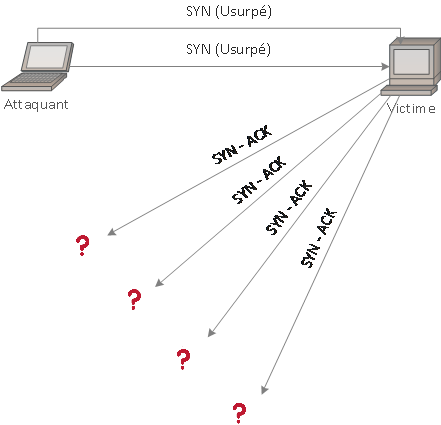
\includegraphics[height=7cm]{IMAGES/ORIGINALS/Attaque_SYN_Flood}
		\end{center}
		\caption{Attaque SYN Flood}
	\end{figure}
	
	Une attaque DDoS SYN flood exploite une faiblesse connue de la séquence de connexion TCP (the « Three-Way Handshake »), dans laquelle une demande SYN pour établir une connexion TCP avec un hôte doit être répondue par une réponse SYN-ACK de cet hôte, et puis confirmé par une réponse ACK du demandeur. Dans un scénario SYN Flood, le demandeur envoie plusieurs demandes SYN à partir d'une adresse IP usurpée, qui ne peut pas répondre à la requête SYN-ACK de l'hôte. Le système hôte continue d'attendre l'accusé de réception pour chacune des demandes, liant les ressources jusqu'à ce qu'aucune nouvelle connexion ne puisse être établie, et entraînant finalement un déni de service.

	\subsubsection{Attaque Smurf}
	\begin{figure}[H]
		\begin{center}
			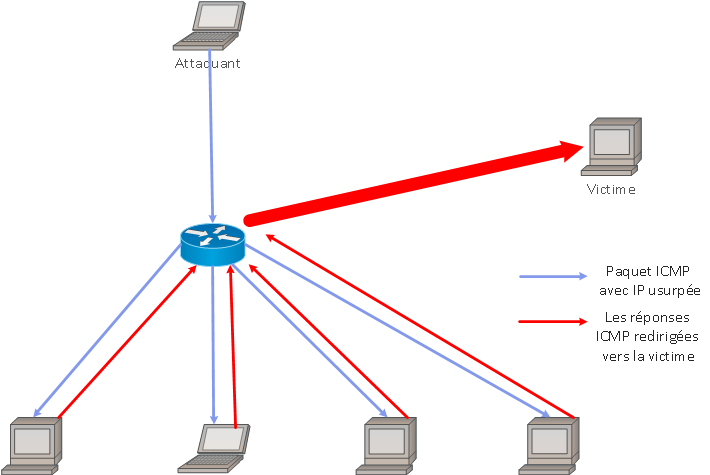
\includegraphics[width=\textwidth]{IMAGES/ORIGINALS/Attaque_Smurf}
		\end{center}
		\caption{Attaque Smurf}
	\end{figure}
		
	Le nom Smurf vient du code source de l'outil d'exploitation original, smurf.c, créé par un individu appelé TFreak en 1997 \cite{ciscoguideagainstddos}. 
Les attaques de Smurf sont quelque peu similaires aux ICMP Flood, car les deux sont effectuées en envoyant une flopée de paquets de demande d'écho ICMP.
Contrairement à ICMP Flood régulière, Smurf est un vecteur d'attaque d'amplification qui augmente son potentiel de dégâts en exploitant les caractéristiques des réseaux de diffusion.\\
	Dans une attaque smurf, un attaquant diffuse un grand nombre de paquets ICMP avec l'adresse IP source usurpée de la victime vers un réseau utilisant une adresse de diffusion IP. Cela oblige les périphériques du réseau à répondre en envoyant une réponse à l'adresse IP source.
	\subsubsection{DNS Flood}
	\begin{figure}[H]
		\begin{center}
			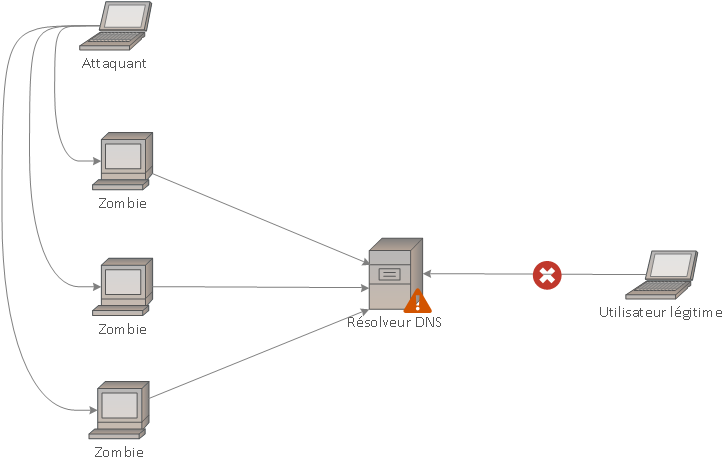
\includegraphics[height=7cm]{IMAGES/ORIGINALS/Attaque_DNS_Flood}
		\end{center}
		\caption{Attaque DNS Flood}
	\end{figure}
	Un DNS Flood est un type d'attaque DDoS où un attaquant submerge les serveurs DNS d'un domaine particulier dans le but de perturber la résolution DNS de ce domaine. Si un utilisateur n'est pas en mesure de trouver le répertoire, il ne peut pas rechercher l'adresse afin d'effectuer l'appel pour une ressource particulière. En perturbant la résolution DNS, une attaque par inondation DNS compromettra la capacité d'un site Web, d'une API ou d'une application Web à répondre au trafic légitime.\\

	Les attaques par inondation DNS utilisent les connexions à large bande passante des caméras IP, d'autres appareils IoT pour submerger directement les serveurs DNS des principaux fournisseurs. Le volume de demandes des appareils IoT submerge les services du fournisseur DNS et empêche les utilisateurs légitimes d'accéder aux serveurs DNS du fournisseur.\\

	Ces attaques DNS diffèrent des attaques par amplification DNS. Contrairement aux inondations DNS, les attaques d'amplification DNS reflètent et amplifient le trafic des serveurs DNS non sécurisés afin de masquer l'origine de l'attaque et d'augmenter son efficacité.	
	\subsection{Attaques volumétriques}
	L’inaccessibilité d’une machine peut être réalisé en surchargeant la bande passante avec des volumes significativement élevés de trafic malveillant. Les attaques DoS et DDoS ciblent directement les réseaux ainsi que leurs périphériques de connexion. Un routeur ne peut traiter qu’une certaine quantité de données à la fois, si cette capacité est dépassée en raison notamment d’une attaque, les services correspondants ne seront alors plus fonctionnels pour les autres utilisateurs.
Les attaques volumétriques sont généralement lancées contre une cible spécifique, généralement des services critiques de fournisseur de services (SP) ou des clients d'entreprise. Les modèles d’attaque sont principalement : ICMP Flood, UDP Flood, IPSec Flood, IP/ICMP Fragmentation, attaques d’amplification de réflexion. 

	\subsubsection{UDP Flood}
	Une UDP Flood est une forme d'attaque volumétrique par déni de service (DoS). Par définition, c’est toute attaque DDoS qui attaque une cible avec des paquets UDP (ne nécessitant pas d’établissement de connexion préalable ou de session). Le but de l'attaque est d'inonder des ports aléatoires sur un hôte distant. Cela oblige l'hôte à vérifier à plusieurs reprises l'application qui écoute sur ce port et (lorsqu'aucune application n'est trouvée) répond avec un paquet ICMP « Destination inaccessible »\cite{impervaddos}. Ce qui conduit à l’inaccessibilité.\\
	Lorsque des attaques par UPD Flood émanent de plusieurs machines, l'attaque est considérée comme une menace de déni de service distribué (DDoS).

	\subsubsection{ICMP Flood}	
	\begin{figure}[H]
		\begin{center}
			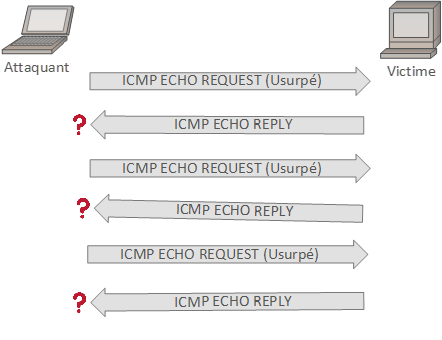
\includegraphics[height=7cm]{IMAGES/ORIGINALS/Attaque_ICMP_Flood}
		\end{center}
		\caption{Attaque ICMP Flood}
	\end{figure}
		
	Similaire en principe à l'attaque UDP Flood, une ICMP Flood submerge la ressource cible avec des paquets de requête d'écho ICMP (ping), envoyant généralement des paquets le plus rapidement possible sans attendre de réponses. Généralement, les messages de demande d'écho et de réponse d'écho ICMP sont utilisés pour envoyer une requête ping à un périphérique réseau afin de diagnostiquer l'intégrité et la connectivité du périphérique et la connexion entre l'expéditeur et le périphérique.\\
	
	Ce type d'attaque peut consommer de la bande passante sortante et entrante, car les serveurs de la victime tentent souvent de répondre avec des paquets de réponse d'écho ICMP, ce qui entraîne un ralentissement global significatif du système. Cette attaque peut être réalisé à l’aide d’outils personnalisé ou code tels que hping and scapy. Elle nécessite au préalable la connaissance de l’adresse IP de la cible.

	\subsubsection{Fragmentation IP/ICMP}
	Une attaque par fragmentation IP/ICMP (soit Internet Protocol / Internet Control Message Protocol) est une forme courante d'attaque volumétrique par déni de service (DoS). Dans une telle attaque, les mécanismes de fragmentation des datagrammes sont utilisés pour submerger le réseau.\\
	Le processus de fragmentation IP est un processus de communication dans laquelle les datagrammes IP sont décomposés en petits paquets, transmis sur un réseau puis réassemblés dans le datagramme d'origine.\\
	La fragmentation est indispensable pour la transmission des données, puisque chaque réseau a une limite unique en matière de taille de datagrammes qu'il peut traiter, qu’on appelle unité de transmission maximale (Maximum Transmission Unit soit MTU). Si le datagramme envoyé est plus grand que le MTU du serveur de réception, il doit être fragmenté pour être transmis complètement.\\

	Dans le cas d’une attaque DoS, l'attaquant peut utiliser la fragmentation IP pour cibler les systèmes de communication, ainsi que les composants de sécurité. Les attaques de fragmentation basées sur ICMP soumettent généralement de faux fragments qui ne peuvent pas être défragmentés. Cela entraîne à son tour le placement des fragments dans un stockage temporaire, occupant de la mémoire et dans certains cas épuisant toutes les ressources de mémoire disponibles.
	\subsubsection{Amplification DNS}
	\begin{figure}[H]
		\begin{center}
			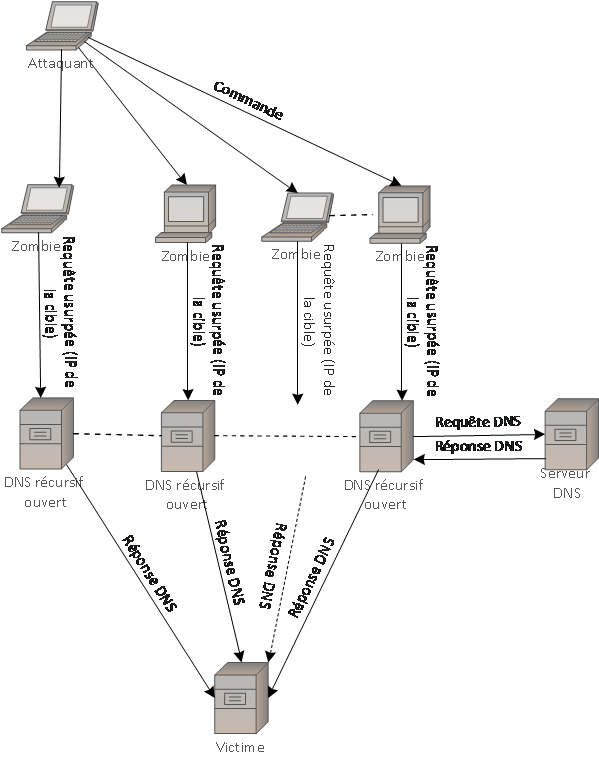
\includegraphics[width=\textwidth,height=15cm]{IMAGES/ORIGINALS/Amplification_DNS}
		\end{center}
		\caption{Architecture d'attaque par amplification DNS}
	\end{figure}	
			
	Les attaques par amplification DNS renforcent la force des attaques de DDoS. Plutôt que d’envoyer le trafic directement d’un botnet à une victime, le botnet envoi des demandes à d’autres systèmes. Ces systèmes répondent en envoyant des volumes de trafic plus importants à la victime. La figure 7 est une illustration de ce type d’attaque.	
	\subsection{Attaques Zero-day}
La définition « Zero-day » englobe toutes les attaques inconnues ou nouvelles, exploitant des vulnérabilités pour lesquelles aucun correctif n'a encore été publié.
En général, le terme attaque Zero-Day (ou attaque 0-day) est utilisé pour les attaques qui utilisent de nouvelles vulnérabilités de sécurité logicielle, dont la communauté n'est pas encore au courant. Cela peut prendre un certain temps entre le moment où le malfaiteur détecte la vulnérabilité et la publication et l'installation du nouveau patch (correctif). Pendant tout ce temps, la vulnérabilité sera activement utilisée pour bloquer les ressources et voler des informations.\\ 

	Par exemple, pour organiser une attaque DDoS réussie, le pirate informatique doit mettre en place un réseau de zombie en peu de temps. La tactique de vulnérabilité Zero-Day est un choix parfait à cet effet. Par conséquent, cette approche gagne en popularité auprès des pirates du monde entier. Pour atteindre leur objectif, les malfaiteurs doivent accéder à un serveur qui exécute un logiciel avec une vulnérabilité de Zero-day. Le serveur peut alors être utilisé pour ce type d'attaques. Cela signifie également qu'il n'est pas nécessaire d'utiliser un grand nombre de machines compromises.\\
	Le terme zero-day est bien connu des membres de la communauté des pirates informatiques, où la pratique du trading de vulnérabilités zero-day est devenue une activité populaire.
	\section{Motivations}
	L'attaques DDoS devient rapidement le type de cyber-menace le plus répandu. Étant donnée la facilité de mises en place des attaques DDoS à faible coût avec très peu de préparation, il est devenu clair que toute organisation court le risque de subir une attaque à tout moment. Mais qu’est-ce qui peut motiver l’auteur d’une attaque ? 
Voici quelques-unes des raisons\cite{bellitddos}.
\subsection{Cyberactivisme}
	Le Cyberactivisme, soit en anglais (Hacktivism). Le DDoS peut servir souvent un mode de protestation contre les sociétés et les gouvernements dont les actions sont considérées comme « incorrectes » ou « mauvaises » par l’attaquant. Par exemple des attaques par des groupes comme Anonymous contre des organisations telles que l’État islamique et le FBI) au personnel et au mesquin (comme des serveurs de jeux informatiques en ligne mis en panne par des joueurs irrités au sujet de changements récents apportés au jeu).
	\subsection{Vandalisme}
	Parfois des attaquants mettent un site Web en panne simplement pour prouver qu’il est possible de le faire, ou pour nulle autre raison que de « se faire remarquer » par une communauté d’utilisateurs en ligne. On attribue ces types d’attaques à ce qu’il est convenu d’appeler des « pirates adolescents » (script kiddies en anglais), en raison de la puérilité des motifs.
	\subsection{Concurrence}
	Si le site Web d’une entreprise donnée tombe en panne, c’est une bonne nouvelle pour ses concurrents. L’entreprise touchée perdra non seulement des ventes, mais sa réputation en prendra également un coup et ses clients pourront affluer vers la concurrence à la place.
	\subsection{Extorsion}
	Les attaquants utilisent des attaques DDoS ou la menace d'attaques DDoS comme moyen d'extorquer de l'argent à leurs cibles. De telles attaques se déroulent souvent de la manière suivante: les attaquants perturbent un site pendant une courte période avec une attaque par déni de service distribué, envoient une note de rançon menaçant de perturber davantage, et si la rançon n'est pas payée, il arrive parfois de faire face à cette menace
	\subsection{Diversion}
	Le DDoS peut également servir de « rideau de fumée » pour dissimuler la véritable cible d’une cyberattaque. Pendant que les équipes de TI s’activent à régler une panne de site Web ou de serveur qui les a détournées de leur attention sur leur vrai travail, il devient plus facile de s’infiltrer furtivement dans le réseau interne de l’entreprise pour lui voler des données financières ou sur ses clients.
\section{Prévention contre les attaques DDoS}
	Les attaques par déni de service distribué (DDoS) représentent une menace importante pour la continuité de l’activité d’un système d’information. Les entreprises, les entités gouvernementales et les particuliers sont devenus de plus en plus dépendantes d’internet, des services web et des applications. La disponibilité de ces systèmes est devenue aussi essentielle que l’électricité.\\

	Les attaques DDoS sont relativement difficile à arrêter, une fois que les machines compromises ont commencé à attaquer la cible. Les conséquences d’une attaque DDoS peuvent être multiples. En effet, la perte de disponibilité d’un service ou d’une application peut provoquer la colère des clients, une perte financière (de revenus) et porté atteinte à l’image de l’entreprise. Lorsque les applications critiques deviennent indisponibles, les opérations et la productivité sont paralysées.\\

	Compte tenu de la nature très médiatisée des attaques par déni de service distribué et de leurs conséquences potentiellement dévastatrices, plusieurs mesures de sécurité ont étés mises au point afin de contrer les surcharges des systèmes de celles-ci.   
Une des solutions peut être d’identifier des adresses IP critiques et de combler les failles de sécurité, par exemple. Ces contre-mesures sont tels que : Ip-Blacklist, filtrage, load balancer, etc.
Des services permettent de contrôler les connexions en amont. Par exemple, Cloudflare qui va mettre l’utilisateur sur une page d’attente pour légitimer ou non sa connexion. Solution viable pour les professionnels.\\

	La principale difficulté pour empêcher une attaque DDoS est de différencier le trafic d'attaque du trafic normal. Par exemple, si un site Web est surchargé de demandes de clients pressés de découvrir la nouvelle version d'un service, ce serait une erreur d'interrompre tout le trafic. En revanche, si cette société connaît brusquement une hausse du trafic provoquée par des acteurs malveillants connus, il est judicieux de prendre des mesures pour limiter l'attaque. Toute la difficulté réside dans le fait qu'il faut distinguer le trafic lié aux clients légitimes de celui provenant de l'attaquant.
	\subsection{Rate limiting}
	La limitation du nombre de demandes qu'un serveur acceptera sur une certaine période est un moyen de réduire les attaques par déni de service. Le rate limiting est utilisé généralement pour contrôler le débit du trafic envoyé ou reçu sur une interface réseau. Toutefois, bien que la limitation du débit soit utile pour ralentir les extracteurs de données Web et atténuer les tentatives de connexion par force brute, seule, elle risque fort d'être insuffisante pour gérer une attaque DDoS complexe efficacement. La limitation du débit reste néanmoins un élément utile dans une stratégie efficace de réduction des attaques DDoS.

	\subsection{Routage de trou noir (blackhole routing)}
	Le routage / filtrage de trou noir DDoS (parfois appelé blackholing) est une contre-mesure pour atténuer une attaque DDoS dans laquelle le trafic réseau est acheminé vers un « trou noir » et est perdu. Lorsque le filtrage du trou noir est mis en place sans critères de restriction spécifiques, le trafic réseau légitime et malveillant est acheminé vers une route nulle ou un trou noir et supprimé du réseau. Lorsque vous utilisez des protocoles sans connexion tels que UDP, aucune notification des données perdues ne sera renvoyée à la source. Avec les protocoles orientés connexion comme TCP, qui nécessitent une prise de contact pour se connecter au système cible, une notification sera renvoyée si les données sont abandonnées. Si un site Internet subit une attaque DDoS, le fournisseur d’accès à Internet (FAI) peut envoyer le trafic entier du site vers un trou noir comme défense.
\subsection{Pare-feu d’application web}
	Un pare-feu d’application web en anglais (Web Application Firewall soit WAF) est un logiciel de traitement de paquets d’état conçu pour arrêter les attaques d’applications basées sur le Web et n’arrête donc pas tous les types d’attaque DDoS tels que les attaques d’épuisement d’état TCP. Toute attaque de réflexion ou d’amplification d’une attaque d’inondation à l’aide de nombreuses sources bot submergerait le WAF et rendrait l’ensemble de la solution inutile. En bref, ces deux technologies sont complémentaires dans leur utilisation pour protéger les organisations contre les attaques, mais un WAF ne protègera pas les vecteurs des attaques DDoS complexes.
Il peut aider à atténuer une attaque DDoS de la couche 7 du modèle OSI. Un atout majeur d’un WAF est sa capacité à mettre en place rapidement des règles personnalisées en réponse à une attaque.
	\section{Conclusion} 
	Les attaques par déni de service distribué (DDoS) se produisent généralement à l’aide d’un botnet. L’attaquant utilise un réseau d’ordinateurs infectés par des logiciels malveillants pour une flopée de trafic vers une cible, comme un serveur. Le but est de surcharger la cible et de ralentir ou de l’écraser.\\
	Les vecteurs d’attaque DDoS sont généralement classés en trois grandes catégories tels que : attaques volumétriques, attaques d’épuisement d’états TCP (TCP state-exhaustion attacks), et attaque de la couche d’application.\\
	L’accès aux services d’une entité doit être restreint afin de n’autoriser que les réseaux internes à celle-ci. Par ailleurs, la mise en place de règles de rate-limiting (limiter le nombre de demandes qu'un serveur acceptera sur une certaine période) peut réduire une éventuelle participation à une attaque par DDoS. Le WAF aussi permet de diminuer les attaques DDoS. Mais la plupart de ces protections classiques sont généralement inefficace face aux attaques DDoS qui sont de plus en plus sophistiquées.\\
	Enfin, le trafic sortant de l’entité doit être filtré afin de bloquer l’envoi de trafic pour lequel les adresses IP sources sont usurpées.

